\chapter{Moduli problems}
    \begin{abstract}
        
    \end{abstract}
    
    \minitoc
    
    \section{Moduli problems and stacks} \label{section: moduli_problems}
        The following conventions shall be followed until the end of the section.
        \begin{convention}
            \noindent
            \begin{itemize}
                \item By $1\-\Cat_1$, or simply $1\-\Cat$, we shall actually mean $(\infty, 1)\-1\-\Cat_1$, i.e. the $(\infty, 1)$-category of $(\infty, 1)$-categories and functors between them, and by $1\-\Cat_2$ we will be referring to the $(\infty, 2)$-category of $(\infty, 1)$-categories, functors between them, and natural transformations between these functors. 
                
                Similarly, by $\Grpd^1$, or simply $\Grpd$, we will actually mean the $(\infty, 1)$-category of $\infty$-groupoids and functors between them, and by $\Grpd^2$, we shall mean the $(\infty, 2)$-category of $\infty$-groupoids, functors between them, and natural transformations between these functors.
                \item A subcategory of $1\-\Cat$ this is of particular interest is $\dg\Cat^{\cont}$, the $(\infty, 2)$-category of stable linear (i.e. differential-graded) $(\infty, 1)$-categories (see section \ref{section: homological_algebra} for the notion of stable $(\infty, 1)$-categories). Of course, we can also view $\dg\Cat^{\cont}$ as a mere $(\infty, 1)$-category.
            \end{itemize} 
        \end{convention}
    
        \subsection{The Grothendieck Construction; fibred categories}
            Alexander Grothendieck, who championed the use of category theory - and in particular, (higher) sheaf theory - in geometry alledgedly said the following when asked about the nature of geometry:
                \begin{center}
                    \say{\textit{To do geometry you really don’t need a space, all you need is a category of sheaves on this space}}
                \end{center}
            and indeed, that was his approach to commutative algebraic geometry: each affine scheme is a representable sheaf on $\Cring^{\op}$, and each scheme, algebraic space, or algebraic stack - by virtue of being locally affine - are nothing but certain colimits of representable sheaves on $\Cring^{\op}$. 
            
            Readers might also be familiar with the other approach to commutative algebraic geometry: one defines a set $|\Spec R|$ consisting of prime ideals of a predetermined commutative ring $R$, equip said set with the so-called Zariski topology, and then recognise that the basic open sets of $|\Spec R|$ are precisely of the form $|\Spec R_f|$ where $f$ represents generators of $R$; from this, one can define topologies finer than the Zariski topology (e.g. \'etale, fppf, etc.), and then sheaves over said topologies, and then so-called \say{schemes} as locally ringed spaces whose structure (pre)sheaves (over the aforementioned topologies) satisfy certain requirements that would force these schemes to be locally affine (for details, see \cite[Chapter 1]{my_commalg_book} or \cite[Chapter 2]{hartshorne}, which is the canonical reference). 
            
            The problem with this latter approach is that while it is very concrete and massively convenient should one wish to do any sort of computation, it also relies heavily on the properties of commutative rings and particularly, how one localises commutative rings at multiplicative submonoids, which do not admit (more-or-less) obvious generalisations to noncommutative and non-associative settings (there have been attempts to define $\Spec A$ for noncommutative or even non-associative algebras $A$, but most are only \say{functorial} for special classes of objects such as $C^*$-algebras); for more details, consult \href{https://mathoverflow.net/questions/159449/why-is-naive-definition-of-non-commutative-spectrum-bad}{\underline{this MO thread}}. On the other hand, the Grothendieckian approach to geometry does not have to succumb to this shortcoming: \say{spaces} are just sheaves, and therefore algebraic data contained in \say{spaces} can be simply encoded in objects of the target category. 
        
            \subsubsection{Universal bundles}
                To expand a bit on the aforementioned perspective of Grothendieck on \say{spaces}, what one wants are so-called \say{moduli stack} of interesting objects. Specifically, what this means is that every morphism in a sufficiently nice category:
                    $$p_x: \E_x \to \calB_x$$
                should arise as some sort of fibre of some \say{universal} morphism:
                    $$p: \E \to \calB$$
                For instance, schemes are \say{good} spaces partly because each point $x \in |X|$ has an associated residue field $\kappa_x$ (whose spectrum, like any other field spectrum, is just a point); then, one can construct fibres $p_x: Y_x \to \Spec \kappa_x$ as pullbacks of morphisms $p: Y \to X$ along the canonical \say{arrow of elements} $x: \Spec \kappa_x \to X$: 
                    $$
                        \begin{tikzcd}
                        	{Y_x} & Y \\
                        	{\Spec \kappa_x} & X
                        	\arrow["{p_x}", from=1-1, to=2-1]
                        	\arrow["x", from=2-1, to=2-2]
                        	\arrow["p", from=1-2, to=2-2]
                        	\arrow[from=1-1, to=1-2]
                        	\arrow["\lrcorner"{anchor=center, pos=0.125}, draw=none, from=1-1, to=2-2]
                        \end{tikzcd}
                    $$
                More generally, one might think of moduli spaces in the classical sense. $\calM_{1, 1 /X}$ - the moduli space of elliptic curves over a base scheme $X$ - is one such space: its fibres over points of $X$ are nothing but elliptic curves over the corresponding residue fields:
                    $$
                        \begin{tikzcd}
                        	{E_x} & {\calM_{1, 1 /X}} \\
                        	{\Spec \kappa_x} & X
                        	\arrow["{p_x}", from=1-1, to=2-1]
                        	\arrow["x", from=2-1, to=2-2]
                        	\arrow["p", from=1-2, to=2-2]
                        	\arrow[from=1-1, to=1-2]
                        	\arrow["\lrcorner"{anchor=center, pos=0.125}, draw=none, from=1-1, to=2-2]
                        \end{tikzcd}
                    $$
                It was these kinds of spaces that inspired Grothendieck to look for a construction for some sort of \say{universal moduli space}, which is now known as the \textbf{Grothendieck Construction}.
                
                \begin{definition}[The Grothendieck Construction] \label{def: grothendieck_construction} \index{Grothendieck Construction}
                    Let ${}^{\pt/}1\-\Cat^{\lax}_2$ denote the $2$-category of so-called \textbf{lax-pointed $1$-categories}:
                        \begin{itemize}
                            \item whose objects are pairs $(\E, e)$ consisting of a category $\E$ and a distinguished object $e$ (recall that a functor from the terminal category $\pt$ is the same as the identification of an object),
                            \item morphisms from $(\E_2, e_2)$ to $(\E_1, e_1)$ are pairs $(f^*, f^{\sharp})$ consisting of a functor $f^*: \E_2 \to \E_1$ along with a morphism $f^{\sharp}: f^*(e_2) \to e_1$ in $\E_1$:
                            \item whose $2$-morphisms are lax-natural transformation between the functors $f^*$.
                        \end{itemize}
                    and note that there is a canonical forgetful functor:
                        $$\oblv: {}^{\pt/}1\-\Cat^{\lax}_2 \to 1\-\Cat_2$$
                    that disregards the choices of distinguished objects and morphisms between them (i.e. $(\E, e)$ gets sent to $\E$). Now, let:
                        $$\beta: \calB \to 1\-\Cat_2$$
                    be any pseudo-functor between weak $2$-categories. Then, the \textbf{Grothendieck Construction} for $\beta$, denoted by $\int \beta$, shall be the folloiwng $2$-pullback:
                        $$
                            \begin{tikzcd}
                            	{\int \beta} & {{}^{\pt/}1\-\Cat^{\lax}_2} \\
                            	\calB & {1\-\Cat_2}
                            	\arrow[from=1-1, to=2-1]
                            	\arrow["\beta", from=2-1, to=2-2]
                            	\arrow["\oblv", from=1-2, to=2-2]
                            	\arrow[from=1-1, to=1-2]
                            	\arrow["2"{description}, "\lrcorner"{anchor=center, pos=0.125}, draw=none, from=1-1, to=2-2]
                            \end{tikzcd}
                        $$
                    Through these Grothendieck constructions, one can view the fibration (exercise!):
                        $$
                            \begin{tikzcd}
                            	{{}^{\pt/}1\-\Cat^{\lax}_2} \\
                            	{1\-\Cat_2}
                            	\arrow["\oblv", from=1-1, to=2-1]
                            \end{tikzcd}
                        $$
                    as a \say{($2$-)universal moduli space}. 
                \end{definition}
                \begin{remark}[Explicit description of Grothendieck Constructions] \label{remark: objects_and_morphisms_of_grothendieck_constructions}
                    
                \end{remark}
                
                \begin{remark}[A review of $2$-adjunctions] \label{remark: 2_adjunctions}
                    \noindent
                    \begin{enumerate}
                        \item \textbf{(Enriched adjunctions and strict $2$-adjunctions):} 
                            \begin{enumerate}
                                \item \textbf{(Enriched adjunctions):} Let $\V$ be a cosmos (i.e. a complete and cocomplete closed symmetric monoidal category) and let $\C, \D$ be two $\V$-enriched categories. Then, a \textbf{$\V$-enriched adjunction}:
                                    $$
                                        \begin{tikzcd}
                                        	\C & \D
                                        	\arrow[""{name=0, anchor=center, inner sep=0}, "R"', shift right=2, from=1-1, to=1-2]
                                        	\arrow[""{name=1, anchor=center, inner sep=0}, "L"', shift right=2, from=1-2, to=1-1]
                                        	\arrow["\dashv"{anchor=center, rotate=-90}, draw=none, from=1, to=0]
                                        \end{tikzcd}
                                    $$
                                is a pair of functors $L: \D \to \C, R: \C \to \D$ such that for all $x \in \C, y \in \D$, we have the following isomorphism in $\V$:
                                    $$\C(Ly, x) \cong \D(y, Rx)$$
                                \item \textbf{(Strict $2$-adjunctions):} By letting $\V$ be $1\-\Cat_1$, one obtains so-called \textbf{strict $2$-adjunctions}, which induces equivalences of $1$-categories of the form:
                                    $$\C(Ly, x) \underset{1}{\cong} \D(y, Rx)$$
                                (again, for all $x \in \C$ and $y \in \D$).
                            \end{enumerate}
                        \item \textbf{(Weak $2$-adjunctions):} Now, what one can do to relax a strict $2$-adjunction into a \textbf{weak $2$-adjunction} (also known as a \textbf{biadjunction}) is to let the enriching cosmos $\V$ be $1\-\Cat_2$ instead of $1\-\Cat_1$. This however, warrants a certain level of care for there to be no circular logical dependence. Particularly, we can not simply define $1\-\Cat_2$ as the category of all $1\-\Cat_1$-enriched categories, as said enriched category would only be a $1$-category: hom-spaces would simply be functor $1$-categories, and no so-called modulators between natural transformations between functors would be taken in account as $2$-morphisms in these functor categories. The way to get around this issue is to instead take $1\-\Cat_2$ as the natural weak $2$-category of (small) categories, anafunctors between said categories, and ananatural transformations between those anafunctors. Then, enriching over $1\-\Cat_2$ would produce \textit{weak} $2$-equivalences of the following form for all $x \in \C$ and $y \in \D$:
                            $$\C(Ly, x) \underset{2, \weak}{\cong} \D(y, Rx)$$
                        \item \textbf{(Lax $2$-adjunctions):} There are also so-called \textbf{lax $2$-adjunctions}. These are not really adjunctions in the usual sense, since they only qualify as \say{adjunctions} up to adjunctions between certain hom-spaces. Particularly, if $(L \underset{2, \lax}{\ladjoint} R)$ is lax $2$-adjoint pair then for all $x \in \C$ and $y \in \D$, we shall have a $1$-adjunction of the following shape:
                            $$
                                \begin{tikzcd}
                                	{\C(Ly, x)} & {\D(y, Rx)}
                                	\arrow[""{name=0, anchor=center, inner sep=0}, "{R_{x, y}}"', shift right=2, from=1-1, to=1-2]
                                	\arrow[""{name=1, anchor=center, inner sep=0}, "{L_{x, y}}"', shift right=2, from=1-2, to=1-1]
                                	\arrow["\dashv"{anchor=center, rotate=-90}, draw=none, from=1, to=0]
                                \end{tikzcd}
                            $$
                    \end{enumerate}
                \end{remark}
                \begin{proposition}[Universal property of the Grothendieck Construction] \label{prop: grothendieck_construction_universal_property}
                    Alternatively (and of course, equivalently), one might define the Grothendieck Construction of pseudo-functors from some base category $\calB$ to $1\-\Cat_2$ as a $2$-functor:
                        $$\int: \Pseudo(\calB, 1\-\Cat_2) \to (1\-\Cat_2)_{/\calB}$$
                    fitting into the following weak $2$-adjunction:
                        $$
                            \begin{tikzcd}
                            	{(1\-\Cat_2)_{/\calB}} & {\Pseudo(\calB, 1\-\Cat_2)} & {}
                            	\arrow[""{name=0, anchor=center, inner sep=0}, "\const"', shift right=2, from=1-1, to=1-2]
                            	\arrow[""{name=1, anchor=center, inner sep=0}, "\int"', shift right=2, from=1-2, to=1-1]
                            	\arrow["\dashv"{anchor=center, rotate=-90}, draw=none, from=1, to=0]
                            \end{tikzcd}
                        $$
                \end{proposition}
                    \begin{proof}
                        
                    \end{proof}
                \begin{corollary}[Grothendieck Constructions are oplax colimits] \label{coro: grothendieck_constructions_are_oplax_colimits}
                    
                \end{corollary}
                
                \begin{definition}[Spaces] \label{def: spaces} \index{Grothendieck Construction}
                    Fix a base category $\calB$. A \textbf{space} over $\calB$, in the largest possible generality, is nothing but a Grothendieck Construction $\E \to \calB$. Note that it satisfies the universal property described in proposition \ref{prop: grothendieck_construction_universal_property} \textit{a priori}. Additionally, note that such a \say{space} comes equipped with transition functors:
                        $$f^*: \E_y \to \E_x$$
                    corresponding to arrows $(f: x \to y) \in \calB$; compositions of these functors satisfy 
                \end{definition}
                \begin{example}[Representable spaces] \label{exmaple: representable_spaces}
                    Let $\calB$ be an arbitrary base category, and consider the Grothendieck Construction whose fibres over objects $x \in \calB$ are the slice categories $\calB_{/x}$. Such a space is said to be \textbf{representable}; note that when it is fibred not in categories but merely sets, it shall be nothing more than a representable presheaf in the conventional sense, thanks to Yoneda's Lemma.
                \end{example}
                
            \subsubsection{Properties of the Grothendieck Construction}
            
            \subsection{Descent theory; stacks}
            
        \subsection{Moduli spaces}
            This subsection, for the most part, is simply a catalogue of terminologies. Our goal is to disambiguate: there are many different yet very similar terminologies in moduli theory, and we would like to clearly state the contexts in which they should be used.
            
            \begin{definition}[Moduli spaces] \label{def: moduli_space} index{Moduli space}
                A \textbf{moduli space} parametrised by a base category $\calB$ is a Grothendiek Construction:
                    $$F: \calM \to \calB$$
                (i.e. \say{space} in the sense of definition \ref{def: spaces}) that is fibred in groupoids, i.e. it is a $2$-pullback of the following form:
                    $$
                        \begin{tikzcd}
                        	{\calM} & {{}^{\pt/}\Grpd^{\lax}_2} \\
                        	\calB & {\Grpd^2}
                        	\arrow[from=1-1, to=2-1]
                        	\arrow["F", from=2-1, to=2-2]
                        	\arrow["\oblv", from=1-2, to=2-2]
                        	\arrow[from=1-1, to=1-2]
                        	\arrow["2"{description}, "\lrcorner"{anchor=center, pos=0.125}, draw=none, from=1-1, to=2-2]
                        \end{tikzcd}
                    $$
            \end{definition}
            \begin{convention} \label{conv: moduli_spaces_in_algebraic_geometry}
                Due to the concept of moduli spaces having originated from algebraic geometry, often times, by saying \say{$\calM \to \calB$ is a moduli space over $\calB$}, we will actually mean \say{$\calM \to \calB$ is a moduli space over $\calB^{\op}$}. If $\calB$ has a terminal object $B$, then we might also say that \say{$\calM$ is a moduli space over $B$}. For instance, a moduli space over a base scheme $B$ is nothing but a Grothendieck Construction fibred in groupoids over $\Sch_{/S}^{\op}$.
            \end{convention}
            We will be following convention \ref{conv: moduli_spaces_in_algebraic_geometry} from now on.
            \begin{remark}[Moduli spaces over small categories] \label{remark: moduli_spaces_over_small_categories}
                If we are to assume the Axiom of Choice, then we will have that every fibred category (i.e. Grothendieck Construction) corresponds to a pseudofunctor. Among other things, this tells us that moduli spaces over small base categories are actually nothing but groupoids internal to the presheaf topos over the same base category. 
            \end{remark}
            \begin{definition}[Fine and coarse moduli spaces] \label{def: fine_and_coarse_moduli_spaces} \index{Moduli space! fine} \index{Moduli space! coarse}
                Let $\calM \to \calB$ be a moduli space over a \textit{small} base category $\calB$. Such a moduli space is said to be \textbf{fine} if and only if it is naturally isomorphic to a representable presheaf; note that fine moduli spaces are therefore skeletal internal groupoids in presheaf topoi. Otherwise, the moduli space is said to be \textbf{coarse}, and because every presheaf can be written as a colimit of representables, every coarse moduli space can be written as a colimit of fine moduli spaces, particularly colimits of diagrams whose edges are all invertible arrows.
            \end{definition} 

    \section{Examples of moduli spaces with arithmetic significance}
        \subsection{Flat descent}
        
        \subsection{Torsors and principal bundles}
            \subsubsection{Torsors}
            
            \subsubsection{An example: Galois descent}
        
        \subsection{Hilbert and Quot schemes}
    
        \subsection{Picard stacks}
            \subsubsection{Line bundles and Picard stacks}
                \begin{definition}[Line bundles] \label{def: line_bundles}
                    \noindent
                    \begin{enumerate}
                        \item \textbf{(Line bundles):} Let $\calY$ be a prestack on $\Cring^{\op}$. Then, a \textbf{line bundle on $\calY$} is a line object (also referred to as an invertible object) in the \textit{symmetric} monoidal category $\QCoh(\calY)$ of quasi-coherent modules on $\calY$ (cf. definition \ref{def: qcoh_def}). For the definition of line objects, see \cite{nlab:line_object}.
                        \item \textbf{(Picard groupoids):} 
                            \begin{enumerate}
                                \item \textbf{(Picard groups ...):} It is not hard to see that given any symmetric monoidal category such as that of quasi-coherent modules over a prestack, isomorphism classes of its line objects (which are non-trivial in general, since monoidal structures are only defined up to coherence isomorphisms) form a group where the multiplication is the monoidal structure. This group is known as the \textbf{Picard group}; we shall denote the Picard group of a prestack $\calY$ on $\Cring^{\op}$ by $\Pic^0(\calY)$. Also, note that Picard groups are trivially abelian.
                                \item \textbf{(... and to categorify them):} However, one might not be content with line bundles forming just a puny group. If that is indeed the case, allow us to introduce the all-new \textbf{weak Picard $2$-group}. The weak Picard $2$-group associated to a given prestack $\calY$ on $\Cring^{\op}$ is first and foremost the category internal to the category $\Grp$ of groups (which we note to have finite pullbacks; see definitions \ref{def: internal_categories} and \ref{remark: internal_categories_alt_def} for an explanation of why this is necessary), whose object of objects is $\Pic^0(\calY)$ and whose object of arrows is the automorphism group $\Aut\left(\Pic^0(\calY)\right)$, which we shall suggestively abbreviate by $\Pic^1(\calY)$:
                                    $$
                                        \begin{tikzcd}
                                        	{\Pic^1(\calY)} & {\Pic^0(\calY)} \\
                                        	{\Pic^0(\calY)}
                                        	\arrow["t"', from=1-1, to=2-1]
                                        	\arrow["s", from=1-1, to=1-2]
                                        \end{tikzcd}
                                    $$
                                Next, observe that the above internal category possesses a natural groupoid structure, owing to the fact that the object of arrows $\Pic^1(\calY)$ is a group (by construction!), which in particular means that every arrow in the internal category $(s, t)$ is invertible, and thus there exists an inversion map:
                                    $$i: \Pic^1(\calY) \to \Pic^1(\calY): \sigma \mapsto \sigma^{-1}$$
                                which trivially fits into the following commutative diagram in $\Grp$ (we shall let the reader check the commutativity of this diagram as an exercise):
                                    $$
                                        \begin{tikzcd}
                                        	{\Pic^1(\calY)} \\
                                        	& {\Pic^1(\calY)} & {\Pic^0(\calY)} \\
                                        	& {\Pic^0(\calY)}
                                        	\arrow["t", from=2-2, to=3-2]
                                        	\arrow["s"', from=2-2, to=2-3]
                                        	\arrow["i"{description}, from=1-1, to=2-2]
                                        	\arrow["s"', from=1-1, to=3-2]
                                        	\arrow["t", from=1-1, to=2-3]
                                        \end{tikzcd}
                                    $$
                                    
                                One important thing to note is that the weak Picard $2$-group $(s, t): \Pic^1(\calY) \toto \Pic^0(\calY)$ is precisely the \href{https://ncatlab.org/nlab/show/core}{\underline{core}} of the full subcategory of $\QCoh(\calY)$ spanned by line bundles, as the automorphisms on $\Pic^0(\calY)$ are precisely the isomorphisms between line bundles on $\calY$, and thus it is also a groupoid in the usual sense (i.e. a groupoid internal to $1\-\Cat$). In particular, this tells us that the weak Picard $2$-group of a prestack is actually strict, and it is for this reason that sometimes we might confuse the terms \say{Picard $2$-group} and \say{Picard groupoid}.
                                
                                From this point on, the Picard $2$-group/groupoid associated to a given prestack $\calY$ shall be denoted simply by $\Pic^1(\calY)$.
                            \end{enumerate}
                    \end{enumerate}
                \end{definition}
                \begin{remark}[A categorical comment] \label{remark: picard_2_groups_are_groups_in_Cat}
                    Because Picard $2$-groups associated to prestacks are strict $2$-groups, they also enjoy the property of being group objects in $1\-\Cat$ and hence in the full subcategory $\Grpd$ thereof. See \cite{nlab:strict_2-group} for more details.
                \end{remark}
                \begin{remark}[Picard groups, Picard $2$-groups, and higher homotopical fairy tales]
                    Fix a prestack $\calY$ on $\Cring^{\op}$.
                    \begin{enumerate}
                        \item \textbf{(Decategorifying Picard $2$-groups):} The underlying set of the Picard group $\Pic^0(\calY)$ can be thought of as the set of connected components of the groupoid $\Pic^1(\calY)$, i.e.:
                            $$\Pic^0(\calY) \cong \pi_0\Pic^1(\calY)$$
                        Intuitively, this should make sense, since the data specifying $\Pic^1(\calY)$ differ from that specifying $\Pic^0(\calY)$ only by the \say{looping} isomorphisms on line bundles on $\calY$, which means that the set of connected components of $\Pic^1(\calY)$ is just the \say{discrete} part, namely the underlying set of $\Pic^0(\calY)$. 
                        \item \textbf{(Higher Picard groups):} For each natural number $n$, let us define the Picard $(n + 1)$-group $\Pic^n(\calY)$ to be the strict $(n + 1)$-group $\Aut^n\left(\Pic^0(\calY)\right)$, where:
                            $$\Aut^n\left(\Pic^0(\calY)\right) \cong \Aut\left( \Aut\left( \cdots \Aut\left(\Pic^0(\calY)\right) \right) \right)$$
                        Of course, for all $r \leq n$, we have:
                            $$\Pic^r(\calY) \cong \pi_r\Pic^n(\calY)$$
                    \end{enumerate}
                \end{remark}
                
                \begin{theorem}[\textit{Hilberts Satz 90}] \label{theorem: hilbert_90}
                    Let $X$ be an arbitrary scheme. Then, one has the following isomorphism of abelian groups:
                        $$\Pic^0(X) \cong H^1_{\tau}(X, \G_m)$$
                    where $\tau \in \{\text{Zariski, smooth, \'etale, fppf}\}$.
                \end{theorem}
                    \begin{proof}
                        
                    \end{proof}
                
                \begin{definition}[Picard prestacks] \label{def: picard_prestacks}
                    Let $k$ be a base commutative ring. Then, let us define the \textbf{Picard stack over $\Spec k$} to be the \href{https://ncatlab.org/nlab/show/core}{\underline{core}} of the full substack:
                        $$\Pic^1: [\Spec k]^{\op} \to \Grpd$$
                    spanned by line bundles of the stack $\QCoh: [\Spec k]^{\op} \to 1\-\Cat$ of quasi-coherent modules on ${}^{k/}\Comm\Alg^{\op}$. That is to say, the Picard prestack associates to each prestack $\calY \in [\Spec k]$, the category $\Pic^1(\calY)$ is the core of the full subcategory of $\QCoh(\calY)$ spanned by line bundles, i.e. nothing but the Picard $2$-group on $\calY$ (cf. definition \ref{def: line_bundles}). Naturally, the Picard prestack is fibred in groupoids, and thus has a shot at being geometric. Also, it is evident that the Picard prestack is a gerbe (cf. convention \ref{conv: prestacks}).
                \end{definition}
            
            \subsubsection{Picard stacks of curves}
            
        \subsection{Moduli stacks of elliptic curves}
            \subsubsection{The geometry of elliptic curves}
                \begin{definition}[Moduli spaces of elliptic curves] \label{def: moduli_of_elliptic_curves} \index{Moduli space! of elliptic curves}
                    \noindent
                    \begin{enumerate}
                        \item \textbf{(Elliptic curves):} An \textbf{elliptic curve} over a given base scheme $B$ is an $B$-scheme:
                            $$E \to B$$
                        that satisfies the following properties:
                            \begin{itemize}
                                \item $E$ is smooth, proper, and of relative dimension $1$ over $B$.
                                \item The fibre of $E$ over any point $x \in |B|$ is a smooth, proper, of pure dimension $1$, and geometric connected over the residue field $\kappa_x$.
                                \item $E$ is a \textit{group $B$-scheme} and as such admits a \textbf{distinguished section} $o_E: B \to E$ as its unit.
                            \end{itemize}
                        In other words, an elliptic curve is an abelian scheme of relative dimension $1$.
                        \item \textbf{(Moduli spaces of elliptic curves):} Over a base scheme $S$, the \textbf{moduli space of elliptic curves} is a prestack:
                            $$(\calM_{1, 1})_{/S}^{\circ}: \Sch_{/S}^{\op} \to \Grpd$$
                        which associates to each $S$-scheme $B$ the \textit{core} (i.e. the maximal subgroupoid) of the category of elliptic curves over $B$ (in the above sense), which we will denote simply by $(\calM_{1, 1})_{/S}^{\circ}(B)$. One thing to note is that the pullback of fibres is given by fibred products, which is to say, given an underlying morphism:
                            $$f: B \to B'$$
                        the pullback along $f$ of an elliptic curve $E' \to B'$ (denoted by $f^*E'$) shall be the elliptic $B$-curve fitting into the following pullback square:
                            $$
                                \begin{tikzcd}
                                	{f^*E'} & {E'} \\
                                	B & {B'}
                                	\arrow[from=1-1, to=2-1]
                                	\arrow["f", from=2-1, to=2-2]
                                	\arrow[from=1-2, to=2-2]
                                	\arrow[from=1-1, to=1-2]
                                	\arrow["\lrcorner"{anchor=center, pos=0.125}, draw=none, from=1-1, to=2-2]
                                \end{tikzcd}
                            $$
                    \end{enumerate}
                \end{definition}
                \begin{remark}[Categories of elliptic curves] \label{remark: categories_of_elliptic_curves}
                    One can also construct the more general moduli \textit{prestack} of elliptic curves, which associates to each $S$-scheme $B$ the category $(\calM_{1, 1})_{/S}(B)$ of elliptic curves over $B$, wherein the morphisms are not necessarily invertible. This prestack, however, is not too much of concern to us, since there is no hope of it being geometric (recall that geometric stacks need to first of all be fibred in groupoids; cf. definition \ref{def: geometric_stacks}).
                \end{remark}
                \begin{remark}[A few supplementary technical comments] \label{remark: moduli_of_elliptic_curves_disambiguations}
                    \noindent
                    \begin{itemize}
                        \item \textbf{(Categories of elliptic curves):}
                            \begin{enumerate}
                                \item \textbf{(Morphisms of elliptic curves):} Fix a base scheme $B$. If one is to use definition \ref{def: moduli_of_elliptic_curves} as one's starting notion of what it means for a scheme to be an elliptic curve, then the morphisms in the category $(\calM_{1, 1})_{/S}(B)$ of elliptic $B$-curves (and hence in its core $(\calM_{1, 1})_{/S}^{\circ}(B)$) are going to be \textit{group $B$-scheme homomorphisms}:
                                    $$
                                        \begin{tikzcd}
                                        	{E_1} && {E_2} \\
                                        	& B
                                        	\arrow[from=1-3, to=2-2]
                                        	\arrow["\phi", from=1-1, to=1-3]
                                        	\arrow[from=1-1, to=2-2]
                                        \end{tikzcd}
                                    $$
                                \item \textbf{(Pullbacks):} It is well-known that thanks to the fact that limits commute, any limit of a group $B$-scheme taken in the ambient category $\Sch_{/B}$ would remain a group $B$-scheme. Is the same true for elliptic $B$-curves ? 
                                
                                To answer this question, one needs to verify that smoothness, properness, the dimension of elliptic curves being $1$, as well as fibres being geometrically connected are all properties stable under (finite) pullbacks. This is rather trivial for smoothness (as well as for relative dimensions) and to a lesser extent, for properness as well (which we recall to be the same as being separated, of finite type, and universally closed), so let us focus on geometric connectedness.
                                
                                Recall first of all that a scheme over a field is geometrically connected if and only if the underlying topological space of any of its geometric fibres is connected.
                            \end{enumerate}
                        \item \textbf{(Group structure on elliptic curves):} 
                            \begin{itemize}
                                \item \textbf{(Group law):} Because limits of group schemes (taken in the ambient category of schemes) are still group schemes, the distinguished section $o_E: B \to E$ of a relative elliptic curve degenerates to a rational point $o_{E_x}: \Spec \kappa_x \to E_x$ (more generally, pullbacks do not interfere with the group structure of an existing elliptic curve). This is the usual \say{point at infinity} or \say{unit point} of an elliptic curve over a field (the residue field $\kappa_x$ in this case).
                                \item \textbf{(Connectedness is important):}
                            \end{itemize}
                    \end{itemize}
                \end{remark}
                
                \begin{proposition}[Base-changing $\calM_{1, 1}^{\circ}$] \label{prop: base_changes_of_moduli_spaces_of_elliptic_curves}
                    Let $\phi: S_2 \to S_1$ be a morphism between two base schemes and let $(\calM_{1, 1})_{/S_1}^{\circ}$ be the  moduli spaces of elliptic curves over $S_1$. Then, there exists a moduli space of elliptic curves $(\calM_{1, 1})_{/S_2}^{\circ}$ fitting into the following pullback square of geometric stacks:
                        $$
                            \begin{tikzcd}
                            	{(\calM_{1, 1})_{/S_1}^{\circ}} & {(\calM_{1, 1})_{/S_1}^{\circ}} \\
                            	{S_2} & {S_1}
                            	\arrow[from=1-2, to=2-2]
                            	\arrow[from=1-1, to=2-1]
                            	\arrow["{\phi}", from=2-1, to=2-2]
                            	\arrow["{}", from=1-1, to=1-2]
                            	\arrow["\lrcorner"{anchor=center, pos=0.125}, draw=none, from=1-1, to=2-2]
                            \end{tikzcd}
                        $$
                \end{proposition}
                    \begin{proof}
                        First of all, the pullback $(\calM_{1, 1})_{/S_2}^{\circ}$ is \textit{a priori} a geometric stack on $\Sch_{/S_2}$. Next, consider a pullback square of the following form in $\Sch_{/S_1}$ (i.e. a pullback between fibres of $(\calM_{1, 1})_{/S_1}^{\circ}$):
                            $$
                                \begin{tikzcd}
                                	{f_1^* E_1} & E \\
                                	{B_1'} & {B_1}
                                	\arrow["{f_1}", from=2-1, to=2-2]
                                	\arrow[from=1-2, to=2-2]
                                	\arrow[from=1-1, to=1-2]
                                	\arrow[from=1-1, to=2-1]
                                	\arrow["\lrcorner"{anchor=center, pos=0.125}, draw=none, from=1-1, to=2-2]
                                \end{tikzcd}
                            $$
                        along with a base change diagram of the following form:
                            $$
                                \begin{tikzcd}
                                	&& {B_2} & {B_1} \\
                                	{B_2'} & {B'_1} & {S_2} & {S_1} \\
                                	{S_2} & {S_1}
                                	\arrow["\phi", from=3-1, to=3-2]
                                	\arrow[from=2-2, to=3-2]
                                	\arrow[from=2-1, to=2-2]
                                	\arrow[from=2-1, to=3-1]
                                	\arrow["\lrcorner"{anchor=center, pos=0.125}, draw=none, from=2-1, to=3-2]
                                	\arrow["\phi", from=2-3, to=2-4]
                                	\arrow[from=3-2, to=2-4]
                                	\arrow[from=3-1, to=2-3]
                                	\arrow["{f_2}", from=2-1, to=1-3]
                                	\arrow["{f_1}", from=2-2, to=1-4]
                                	\arrow[from=1-3, to=1-4]
                                	\arrow[from=1-4, to=2-4]
                                	\arrow[from=1-3, to=2-3]
                                	\arrow["\lrcorner"{anchor=center, pos=0.125}, draw=none, from=1-3, to=2-4]
                                \end{tikzcd}
                            $$
                        Pulling the first diagram back along $\phi: S_2 \to S_1$ (using the second diagram as a guide in the process) thus yields:
                            $$
                                \begin{tikzcd}
                                	{\phi^* f_1^* E_1} & {\phi^*E_1} \\
                                	{B_2'} & {B_2} & {f_1^* E_1} & {E_1} \\
                                	&& {B'_1} & {B_1}
                                	\arrow[from=2-1, to=3-3]
                                	\arrow["{f_2}", from=2-1, to=2-2]
                                	\arrow["{f_1}", from=3-3, to=3-4]
                                	\arrow[from=2-2, to=3-4]
                                	\arrow[from=2-4, to=3-4]
                                	\arrow[from=1-2, to=2-2]
                                	\arrow[from=1-2, to=2-4]
                                	\arrow[from=2-3, to=2-4]
                                	\arrow[from=2-3, to=3-3]
                                	\arrow[from=1-1, to=2-1]
                                	\arrow[from=1-1, to=1-2]
                                	\arrow[from=1-1, to=2-3]
                                	\arrow["\lrcorner"{anchor=center, pos=0.125}, draw=none, from=2-3, to=3-4]
                                	\arrow["\lrcorner"{anchor=center, pos=0.125}, draw=none, from=1-1, to=2-2]
                                \end{tikzcd}
                            $$
                        We know \textit{a prioi} that $f_1* E_1$ and $\phi^* f_1* E_1$ must be elliptic curves, and with this, the proof is done.
                    \end{proof}
                
                \begin{proposition}[$\calM_{1, 1}^{\circ}$ is a geometric stack] \label{prop: moduli_stacks_of_elliptic_curves}
                    Let $S$ be a base scheme. Then, the moduli space of elliptic curves $(\calM_{1, 1})_{/S}^{\circ}$ is a geometric stack on $\Sch_{/S, \tau}$, where:
                        $$\tau \in \{\text{Zariski, \'etale, fppf, fpqc}\}$$
                    is a Grothendieck topology on $\Sch_{/S}$.
                \end{proposition}
                    \begin{proof}
                        We will take definition \ref{def: schemes} as our working definition of schemes. It will become clear in a moment why this is necessary.
                        \begin{enumerate}
                            \item \textbf{(Descent satisfaction):} The sheaf condition (up to invertible $2$-cells, of course) is an easy consequence of the fact that pullbacks of elliptic curves along arrows $f: B \to B'$ in $\Sch_{/S}$ are given by fibred products (cf. definition \ref{def: moduli_of_elliptic_curves}).
                            \item \textbf{(A smooth atlas):} 
                            \item \textbf{(Schematicity of the diagonal):} 
                        \end{enumerate}
                    \end{proof}
            
            \subsubsection{The arithmetic of elliptic curves}  
                \paragraph{Level structures on the moduli stack of elliptic curves}
            
                \paragraph{Good and bad reductions}
                    \begin{definition}[Models] \label{def: local_models_of_varieties} \index{Model! of an algebraic scheme}
                        Let $R$ be a discrete valutation ring with fraction field $K$ and let $X$ be an algebraic scheme $\Spec K$ (i.e. a scheme of finite type over $\Spec K$); often, $X$ will be a variety instead of a mere algebraic scheme. A \textbf{model for $X$ over a $\Spec R$} is a \textit{flat} and of \textit{finite type} $\Spec R$-scheme $\bbX$ whose pullback along the canonical arrow $\Spec K \to \Spec R$ is (isomorphic to) $X$, i.e. one fitting into the following pullback square:
                            $$
                                \begin{tikzcd}
                                	X & \bbX \\
                                	{\Spec K} & {\Spec R}
                                	\arrow[from=1-1, to=2-1]
                                	\arrow[from=2-1, to=2-2]
                                	\arrow[from=1-2, to=2-2]
                                	\arrow[from=1-1, to=1-2]
                                	\arrow["\lrcorner"{anchor=center, pos=0.125}, draw=none, from=1-1, to=2-2]
                                \end{tikzcd}
                            $$
                        In other words, a model for an algebraic scheme $X$ over the field of fractions $K$ of some discrete valuation ring $R$ is just a scheme $\bbX$ over $\Spec R$ whose generic fibre is precisely $X$. 
                        
                        One can also impose adjectives such as \say{smooth}, \say{\'etale}, or \say{proper} onto models of algebraic schemes, as long as morphisms characterised by these adjectives are flat and of finite type. If $P$ is a property described by one such adjective, then we say that a model $\bbX \to \Spec R$ is $P$ if and only if the morphism $\bbX \to \Spec R$ is $P$.
                    \end{definition}
                
                    \begin{definition}[Good and bad reductions] \label{def: reductions}
                        Let $X$ be an algebraic scheme over the field of fractions $K$ of a discrete valuation ring $R$, and let $\varpi \in R$ be a uniformiser (i.e. a generator of the unique maximal ideal of $R$). 
                        \begin{enumerate}
                            \item \textbf{(Good/bad reductions):} A reduction modulo $\varpi$ (or in other terminologies, at place $\varpi$) of a model $\bbX \to \Spec R$ of $X$ is just the pullback along the canonical morphism $\Spec R/\varpi \to \Spec R$ of $\bbX \to \Spec R$. It is called \textbf{good} if it is smooth or \say{better} (for instance, \'etale fibres can be considered good reductions). Otherwise, it is called \textbf{bad}.
                            
                            One thing to note is that smooth models and better ones \textit{a priori} have good reductions, since smoothness (and say, \'etale-ness) is preserved under arbitrary base changes (cf. proposition \ref{prop: compositions_and_base_changes_of_smooth_morphisms} and corollary \ref{coro: compositions_and_base_changes_of_etale_morphisms}).
                            \item \textbf{(Places of reduction):} Let $\varpi$ be a generator of the unique and (necessarily) principal maximal ideal of the discrete valuation ring $R$ (or equivalently, denote the unique and principal maximal ideal of $R$ by $(\varpi)$). An algebraic $K$-scheme $X$ is said to have a \textbf{place $\varpi$ of good reduction} if and only if there exist an $R$-model $\bbX \to \Spec R$ of $X$ whose reduction modulo $\varpi$ is good. One might also phrase things geometrically and say that $X$ has good reduction at the closed point $\Spec R/\varpi$.
                            
                            $X$ is said to have a \textbf{place $\varpi$ of bad reduction} if and only if there does not exist an $R$-model $\bbX \to \Spec R$ of $X$ whose reduction modulo $\varpi$ is good (or equivalently, if and only if the reduction modulo $\varpi$ of all $R$-models of $X$ are bad).
                            
                            For more information on so-called \say{places} and prime ideals, see convention \ref{conv: places_and_primes}.
                        \end{enumerate}
                    \end{definition}
                    \begin{example}[Reduction modulo $p$ of curves over $\Q$]
                        Let $p$ be a prime, and note firstly that $\Z_{(p)}$ is a discrete valuation ring by virtue of being a local PID that is not a field; its unique maximal ideal is $(p)$ (and hence one can take $p$ to be a uniformiser), as every element that is not equivalent to $0$ modulo $p$ has already been made to be invertible in $\Z_{(p)}$. Let $X$ be a smooth projective curve over $\Spec \Q$, and let $\bbX_{(p)} \to \Spec \Z_{(p)}$ be a model of $X$ (due to the Fundamental Theorem of Arithmetic, $\Z_{(p)}$ is has $\Q$ as its field of fractions). Then, a reduction modulo $p$ of $X$ is nothing but a fibre product $\bbX_{(p)} \x_{\Spec \Z_{(p)}} \Spec \F_p$. 
                    \end{example}
                    \begin{remark}[Locality of reduction]
                        It is worth noting that a curve $X \to \Spec K$ having good reduction at a place $\varpi$ is a local phenomenon. That is to say, a curve may have good reductions at all places $\varpi$ (for instance, there might be curves over $\Q$ such that all of their $\Z_{(p)}$ possess good modulo $p$ reductions), but the equation defining said curve may be singular in some manner after reduction modulo $\varpi$. 
                    \end{remark}
                    
                    \begin{lemma}[Existence of smooth models]
                        Let $R$ be a discrete valuation ring with field of fraction $K$. Then, there exist a flat, of finite presentation, and proper $R$-model $\bbX$ for any smooth scheme $X$ over $\Spec K$.
                    \end{lemma}
                        \begin{proof}
                            
                        \end{proof}
                    
                    \begin{theorem}[Shimura '55]
                        Let $X$ be a smooth projective variety over $\Spec \Q$. Then $X$ has finitely many places of bad reduction. That is to say, there are only finitely many places $p$ at which the reduction modulo $p$ of a $\Z_{(p)}$-model of $X$ is bad.
                    \end{theorem}
                        \begin{proof}
                            
                        \end{proof}
                    \begin{example}
                        \noindent
                        \begin{enumerate}
                            \item \textbf{(A cubic curve with places of bad reduction):} Consider the cubic curve given by the polynomial equation $x^3 - y^2  - 2 = 0$ (or in other words, consider the variety $X := \Spec \frac{\Q[x, y]}{(x^3 - y^2)}$), which we note to be smooth over $\Q$. Let $\bbX_{(p)}$ be a model over $\Spec \Z_{(p)}$ of $X$. Then, reductions modulo $p$ of $\bbX_{(p)}$ will remain smooth (i.e. good) at all places except at $p = 2$, because:
                                $$x^3 - y^2 - 2 \equiv x^3 - y^2 \pmod{2}$$
                            meaning that the reduction modulo $2$ of $\bbX_{(2)}$ has a cusp at the origin, and at $p = 3$, since:
                                $$x^3 - y^2 - 2 \equiv (x - 2)^3 - y^2 \pmod{3}$$
                            meaning that the reduction modulo $3$ of $\bbX_{(3)}$ has a cusp at $(x, y) = (2, 0)$.
                            \item \textbf{(Reductions of $p$-adic elliptic curves \cite[Example 5.2]{silverman_elliptic_curves}):} Let $p \geq 5$ be a prime and let $E_1, E_2$ be elliptic curves over $\Q_p$ that are given by the equations:
                                $$x^3 + px^2 - y^2 + 1 = 0$$
                            and:
                                $$x^3 - y^2 + p = 0$$
                            We know from the previous example that the second curve is cuspidal at place $p$, so let us focus our attention on the first curve. Reducing modulo $p$ gives a curve determined by the following equation:
                                $$x^3 - y^2 + 1 = 0$$
                            which we note to be smooth, and thus the place $p$ is of good reduction. The assumption that our prime $p$ is larger than or equal to $5$ is crucial for $p$ to be a place of good reduction for $E_1$, because when $p = 2$ or $p = 3$, the equation of the curve obtained after reduction modulo $p$ will be:
                                $$\text{$x^3 - (y + 1)^2 = 0$ or $(x - 1)^3 - y^2 = 0$}$$
                            and both are cuspidal.
                            \\
                            Over $\Q_p(\sqrt[6]{p})$, however, the curve $E_2$ does have good reduction at $p$: by setting $x = \sqrt[3]{p} s$ and $y = \sqrt[2]{p} t$, one gets the following equivalent equation defining the curve $E_2$:
                                $$ps^3 - pt^2 + p = 0$$
                            which becomes the trivial equation $0 = 0$ after reduction modulo $p$. 
                            \item \textbf{(Reduction of smooth projective $p$-adic surfaces):} Let $p$ be an arbitrary prime, let $K$ be a $p$-adic field (i.e. a finite extension of $\Q_p$), and let $X$ be a conic bundle over $\P^1_K$ with four degenrate fibres. First of all, note that $X$ is a smooth projective variety over $\Spec K$ whose $\ell$-adic cohomologies (with $\ell$ any prime distinct from $p$) are all unramified (cf. definition \ref{def: ramification_indices}). Second of all, by being a conic bundle, $X$ is $\overline{K}$-birational to $\P^1_K$. 
                            \item \textbf{(Reduction of abelian varieties):} Let $A$ be an abelian variety over $\Spec \Q$ and let $p, \ell$ be distinct primes. Then, by \cite[Theorem 1.1.1]{conradbrinon}, there exists a $\Z_{(p)}$-model of $A$ with good reduction at $p$ if and only if the $\ell$-adic \'etale cohomologies of $A$ are all unramified at $p$. A special case of this phenomenon is theorem 7.1 of \cite{silverman_elliptic_curves}, which gives a criterion by N\'eron-Ogg-Shafarevich for when elliptic curves admits good reduction at $p$;  
                        \end{enumerate}
                    \end{example}
                    
                    \begin{remark}[Global models ?] \label{remark: global_models}
                        Let $p$ be a prime, let $\bbX_p \to \Spec \Z_p$ model of some $p$-adic algebraic scheme $X_p \to \Spec \Q_p$, and suppose that for whatever reason, we want to be able lift this scheme to $\Q$; $X$ could be some sort of smooth projective geometrically connected curve and we might want to understand the compatibility of local and global class field theory via its \'etale fundamental group for example (for such a purpose, we would also want to be able to \say{localise} to $\Q_p$ from $\Q$), or perhaps we would want to check multiple primes and see where a given smooth curve has bad reductions. Then, even though $\Q$ is the same as the fraction field of say, $\Z_{(p)}$, we can use the fact that it is also the field of fractions of $\Z$ to construct some sort \say{global} model $\bbX_0 \to \Spec \Z$. The algebraic scheme $X_0 \to \Spec \Q$ be an object over the generic fibre $(0) \in |\Spec \Z|$, whereas $X_p \to \Spec \Q_p$ would be a \say{local} object over the special fibre $(p) \in |\Spec \Z|$.  
                            \begin{figure}[H]
                                \centering
                                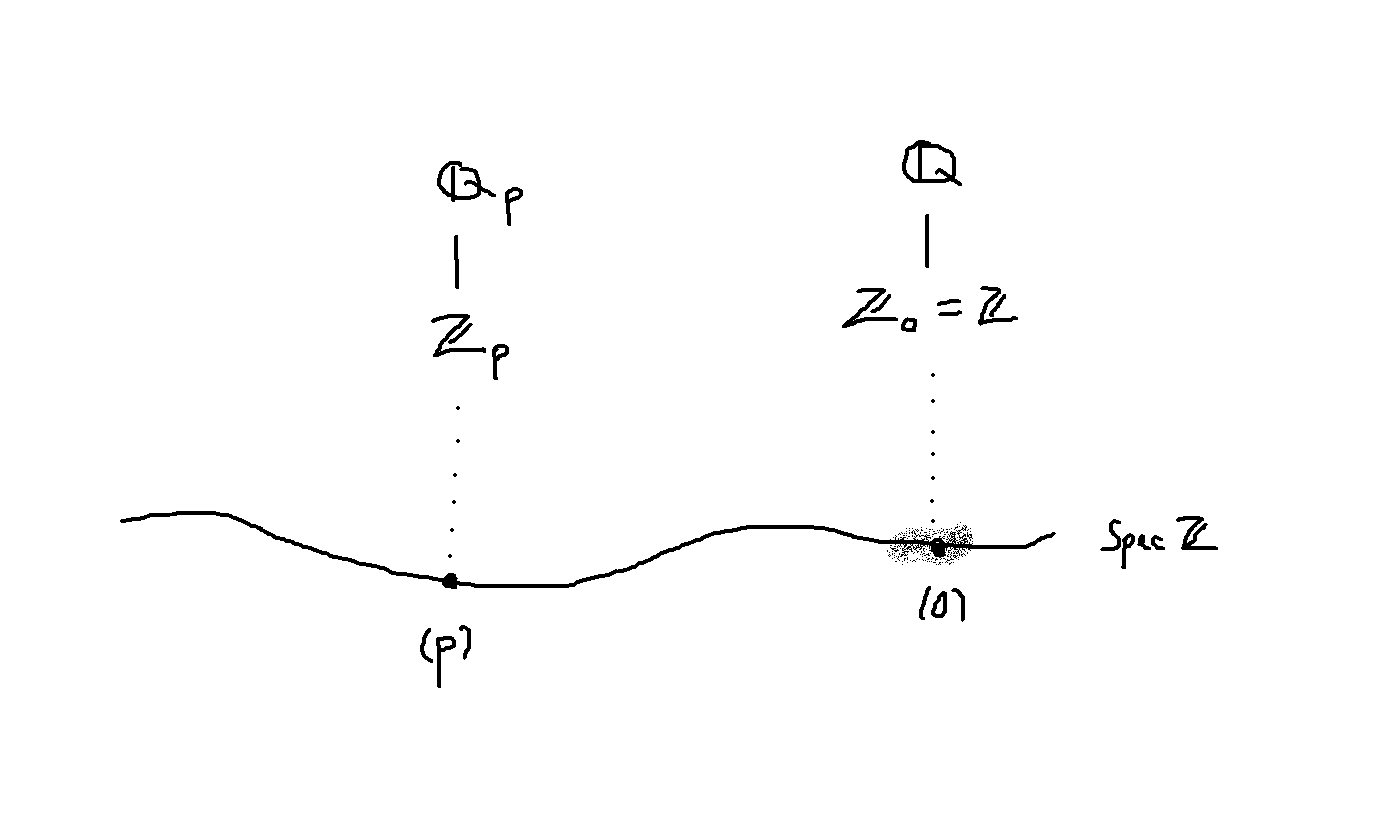
\includegraphics[width=\linewidth,height=\textheight,keepaspectratio]{Figures/places of Spec Z.png}
                                \caption{Local and global points of $\Spec \Z$}
                                \label{fig: local_and_global_points_of_Spec_Z}
                            \end{figure}
                    \end{remark}
                    \begin{definition}[Global models] \label{def: global_models}
                        We want our parametrising scheme, like $\Spec \Z$, to be one where the infinitestimal neighbourhoods (i.e. formal completions) around correspond to spectra of complete discrete valuation rings (for instance, the infinitestimal neighbourhoods $\Spf \Z_p$ around the points $(p) \in |\Spec \Z|$ correspond uniquely to the affine schemes $\Spec \Z_p$), which essentially means we want . We also want $S$ to be connected so that any residue field at a generic point would automatically be the function field of $S$.
                        
                        Let $S$ be base scheme satisfying the above conditions and let $K_0$ be its function field. Then, a \textbf{global model} for an algebraic scheme $X_0$ over $K_0$ shall be a flat and of finite type $S$-scheme $\bbX_0 \to S$. 
                    \end{definition}
                    \begin{remark}[Local-global compatibility] \label{remark: global_to_local_for_models}
                        
                    \end{remark}
                    
                    \begin{definition}[Pointed curves] \label{def: pointed_curves}
                        A \textbf{pointed elliptic curve} is a \textit{finitely presented} and \textit{proper} global model:
                            $$\bbE_0 \to S$$
                        with a distinguised so-called unit section $o_{\bbE_0}: S \to \bbE_0$ of one of the following:
                            \begin{itemize}
                                \item an elliptic curve over a place of $S$,
                                \item a projective nodal cubic curve over a place of $S$ (cf. \cite[\href{https://stacks.math.columbia.edu/tag/0C46}{Tag 0C46}]{stacks}), or
                                \item a projective cuspidal cubic curve over a place of $S$ (a point is a cusp if it corresponds to a non-splitting prime with inertial degree $2$; cf. definition \ref{def: ramification_indices}). 
                            \end{itemize}
                        A fibre of the first kind is said to be over a place of \textbf{good reduction}, whereas fibres over places of the second and third kind are said to be of \textbf{bad reduction}, as one ends up with singularities at those places.
                    \end{definition}
        
        \subsection{Moduli spaces of higher-dimensional abelian varieties; Shimura varieties}
            In a toungue-in-cheek manner, one might say that elliptic curves are nothing but abelian varieties of dimension $1$. One would not be in saying so, but in describing elliptic curves that way, one masks too many important aspects of these objects. This point of view is not entirely myopic and overly simplistic, however, since it does lead to a very fundamental question: do moduli spaces of higher-dimensional abelian varieties admit reasonable descriptions ? To answer this, let us note beforehand that elliptic curves are more than just $1$-dimensional abelian varieties: they admit \textbf{P}olarisations, \say{interesting} \textbf{E}ndomorphism rings, and \textbf{L}evel structures. As moduli stacks of elliptic curves with these extra structures taken into consideration behave quite well, geometrically, speaking, it thus makes sense to consider moduli spaces of abelian varieties that admitting these structures, so-called \textbf{\textit{PEL}-type abelian varieties} (note that elliptic curves admit polarisations trivially, as their automorphism groups - assuming the base field is of characteristic $p \not = 2, 3$ - are isomorphic to $\Z/n\Z$ for $n \in \{2, 4, 6\}$, i.e. finite). 
            
            \subsubsection{The geometry of abelian varieties}
                \begin{definition}[Abelian varieties] \label{def: abelian_varieties}
                    Fix a base scheme $S$. An \textbf{abelian $S$-scheme} is a group $S$-scheme that is smooth, proper, and geometrically connected. An abelian scheme over a field is \textit{a priori} an algebraic variety (in the sense of definition \ref{def: varieties}), so we shall refer to it as an \textbf{abelian variety}.
                \end{definition}
                This might seem like a rather stupid definition: abelian schemes sound like they should be abelian groups in the category of schemes, so why have we not just declared that every abelian group internal to $\Sch_{/S}$ is an abelian scheme ? The reason is two-fold:
                    \begin{enumerate}
                        \item By requiring that our abelian varieties are smooth and proper, we ensure that the machineries of \'etale cohomology are applicable.
                        \item Abelian group objects in $\Sch_{/S}$ can be geometrically very pathological. For instance, the group scheme associating to any commutative $\F_p$-algebra $R$ (for some prime $p$) its group of $n^{th}$ roots of unity is certainly commutative ($\mu_n(R)$, after all, is necessarily a subgroup of $\Z/n\Z$), which is represented by the affine scheme $\Spec \F_p[\zeta]/(\zeta^n - 1)$, is not even smooth in general, as the associated Jacobian vanishses everywhere (cf. definition \ref{def: standard_smoothness}).
                    \end{enumerate}
                As for why we have required abelian schemes to be geometrically connected group schemes in addition to being smooth and proper, this is because we want to make sure that elliptic curves are special cases of abelian schemes (in fact, elliptic curves are precisely abelian schemes of dimension $1$). Additionally, we will see how the connectedness assumption will help us prove that abelian schemes are indeed commutative group schemes.
                
                \begin{remark}[Basic geometric facts about abelian varieties] \label{remark: geometry_of_abelian_varieties}
                    \noindent
                    \begin{itemize}
                        \item \textbf{(Stability under base change):} If $A \to S$ is any ablian scheme and $S' \to S$ is an arbitrary morphism then $A' \cong S' \x_S A$ will also be an abelian scheme, albeit over $S'$ instead of $S$ this time. The proof of this assertion is identical to the argument presented in \ref{remark: moduli_of_elliptic_curves_disambiguations}.
                        \item \textbf{(Moduli stacks of abelian schemes):} For every fixed base scheme $S$, there exists a natural category of abelian $S$-schemes, wherein:
                            \begin{itemize}
                                \item the objects are abelian $S$-schemes, and
                                \item the morphisms are group scheme homomorphisms over $S$.
                            \end{itemize}
                        We will denote it by $(\calM_{n \geq 1})_{/S}$ (where the \say{$n \geq 1$} suggests that abelian of dimensions possibly higher than $1$ are also included); we choose this notation instead of $\Ab(S)$ to avoid confusing abelian schemes with abelian groups internal to schemes. Interestingly, not only is this a full subcategory of the category spanned by (smooth, proper, and geometrically connected) group schemes over $S$, but it is also fibred (in groupoids) over $\Sch_{/S}$ via the evident forgetful functor: the pullback functors between the fibres are simply given by fibred products. Furthermore, the aforementioned fibration:
                            $$(\calM_{n \geq 1})_{/S} \to \Sch_{/S}$$
                        satisfies Zariski, \'etale, fppf, and fpqc descent. 
                        
                        Now, for reasons similar to those discussed in remark \ref{remark: categories_of_elliptic_curves}, we will actually be more interested in the core of the category of abelian $S$-schemes, which we shall denote by $(\calM_{n \geq 1})_{/S}^{\circ}$. This category is (tautologically) fibred in groupoids over $\Sch_{/S}$, and later on, we shall show that certain subcategories of it admits meaningful geometric interpretations.
                        \item \textbf{(Integrality):}
                    \end{itemize}
                \end{remark}
                
                \begin{theorem}[Rigidity of proper flat families] \label{theorem: rigidity_theorem_1}
                    Let $\pi: X \to S$ be a flat and proper morphism of schemes whose local $0^{th}$ cohomologies are all isomorphic to the corresponding residue fields, i.e.:
                        $$\forall s \in |S|: H^0(X_s, \calO_{X_s}) \cong \kappa_s$$
                    Then:
                        \begin{enumerate}
                            \item the canonical map $\pi^{\sharp}: \calO_S \to \pi_*\calO_X$ will be an isomorphism, and
                            \item if $f: S' \to S$ is an affine-schematic morphism and if $\pi': X' \to S'$ is any morphism making the following diagram commutative:
                                $$
                                    \begin{tikzcd}
                                    	{X'} & X \\
                                    	{S'} & S
                                    	\arrow["f", from=2-1, to=2-2]
                                    	\arrow["\pi", from=1-2, to=2-2]
                                    	\arrow["{\pi'}"', from=1-1, to=2-1]
                                    	\arrow[from=1-1, to=1-2]
                                    \end{tikzcd}
                                $$
                            then $\pi': X' \to S'$ shall be constant.
                        \end{enumerate}
                \end{theorem}
                    \begin{proof}
                        \noindent
                        \begin{enumerate}
                            \item 
                            \item 
                        \end{enumerate}             
                    \end{proof}
                \begin{corollary} \label{coro: rigidity_theorem_2}
                    Let $\pi_1: X \to S$ be a flat and proper morphism of schemes whose local $0^{th}$ cohomologies are all isomorphic to the corresponding residue fields, i.e.:
                        $$\forall s \in |S|: H^0(X_s, \calO_{X_s}) \cong \kappa_s$$
                    Additionally, let $\pi_2: Y \to S$ be a separated map fitting into the following commutative diagram:
                        $$
                            \begin{tikzcd}
                            	X && Y \\
                            	& S
                            	\arrow["{\pi_1}"', from=1-1, to=2-2]
                            	\arrow["{\pi_2}", from=1-3, to=2-2]
                            	\arrow["f", from=1-1, to=1-3]
                            \end{tikzcd}
                        $$
                    Suppose now that $f: X \to Y$ is such that the fibre $f_s: X_s \to Y_s$ is constant for some fixed $s \in |S|$. Then, the restriction of $f: X \to Y$ to the connected component of the given point $s \in |S|$ will also be constant.
                \end{corollary}
                    \begin{proof}
                        
                    \end{proof}
                \begin{corollary}[Abelian schemes are abelian groups] \label{coro: abelian_schemes_are_abelian_groups}
                    Abelian schemes are abelian group objects in schemes.
                \end{corollary}
                    \begin{proof}
                        
                    \end{proof}
                    
            \subsubsection{The arithmetic of abelian varieties}
                \paragraph{Polarisations}
                    Let us first take a look at the moduli stack of polarised schemes. For that, however, we will need to say what it means for a line bundle on a scheme to be relatively ample beforehand.
                    
                    The following definition is actually not the most general one (cf. \cite[\href{https://stacks.math.columbia.edu/tag/01VG}{Tag 01VG}]{stacks}), but since abelian schemes are proper by definition, and most base schemes in arithmetic geometry are Noetherian anyway (in fact, most of the time one will simply be working over the spectrum of a field or a very topologically \say{nice} ring like $\Z$ or $\Z_p$), this notion of relative ampleness will suffice.
                    \begin{definition}[Relatively ample line bundles] \label{def: relatively_ample_line_bundles}
                        Let $\pi: X \to S$ be a morphism of schemes, and let $\calL$ be an invertible line bundle over $\calO_{X/S}$. This is said to be \textbf{$\pi$-relatively ample} if and only if:
                            \begin{itemize}
                                \item the base scheme $S$ is Noetherian,
                                \item the structural morphism $\pi: X \to S$ is proper, and
                                \item there exists $s \geq 0$ such that for all $\calF \in \Coh(X_{/S})$, all the higher cohomologies of $\calF \tensor_{\calO_{X/S}} \calL^{\tensor r}$ vanish for $r \geq s$, i.e.:
                                    $$\exists s \geq 0: \forall i > 0: \forall r \geq s: H^i(X_{/S}, \calF \tensor \calL^{\tensor r}) \cong 0$$
                            \end{itemize}
                    \end{definition}
                    \begin{remark}[Base-changing ample line bundles] \label{remark: base_changing_ample_line_bundles}
                        Let $S$ be a Noetherian base scheme, let $\pi: X \to S$ be a proper morphism, and let $f: S' \to S$ be a morphism of finite presentation. Next, consider the following pullback square:
                            $$
                                \begin{tikzcd}
                                	{X'} & X \\
                                	{S'} & S
                                	\arrow["g", from=1-1, to=1-2]
                                	\arrow["{\pi'}"', from=1-1, to=2-1]
                                	\arrow["\pi", from=1-2, to=2-2]
                                	\arrow["f", from=2-1, to=2-2]
                                	\arrow["\lrcorner"{anchor=center, pos=0.125}, draw=none, from=1-1, to=2-2]
                                \end{tikzcd}
                            $$
                        Also, suppose that $\calL$ is a $\pi$-relatively ample line bundle on $X/S$. Now, note that because $f: S' \to S$ is of finite presentation, $\calO_{S'}$ has to be coherent as a $\calO_S$-module, and hence $\calO_{X'}$ is coherent over $\calO_X$ as well. This implies, via the ampleness assumption on $\calL$, that for all coherent $\calO_{X'}$-modules $\calF'$, there exists $s \geq 0$ such that:
                            $$\forall i' > 0: \forall r' \geq s': H^i\left(X'_{/S'}, \calF' \tensor_{\calO_{X'}} \left(\calL^{\tensor r'} \tensor_{\calO_X} \calO_{X'}\right)\right) \cong 0$$
                        This tells us that the obvious base change $g^*\calL \cong \calL \tensor_{\calO_X} \calO_{X'}$ is indeed $\pi'$-relatively ample.
                    \end{remark}
                    
                    We can now define polarisations on schemes:
                    \begin{definition}[Polarisations] \label{def: polarisations}
                        Let $S$ be a Noetherian base scheme and consider a pullback square of the following form:
                            $$
                                \begin{tikzcd}
                                	{X'} & X \\
                                	{S'} & S
                                	\arrow["g", from=1-1, to=1-2]
                                	\arrow["{\pi'}"', from=1-1, to=2-1]
                                	\arrow["\pi", from=1-2, to=2-2]
                                	\arrow["f", from=2-1, to=2-2]
                                	\arrow["\lrcorner"{anchor=center, pos=0.125}, draw=none, from=1-1, to=2-2]
                                \end{tikzcd}
                            $$
                        wherein $\pi: X \to S$ and is flat, proper, and of finite presentation (and hence so is $\pi': X' \to S'$). If $\calL$ and $\calL'$ are relatively ample line bundles on $X/S$ and $X'/S'$ respectively, then one says that they define a \textbf{polarisation between $X/S$ and $X'/S'$} if and only if:
                            $$\calL' \cong g^*\calL$$
                    \end{definition}
                    \begin{remark}[Moduli stackss of polarised schemes] \label{remark: moduli_stacks_of_polarisations}
                        There is a natural fppf-stack of polarised flat proper schemes, which is in fact a substack of the relative Picard stack over $S$, which, we recall, classifies line bundles over $S$-schemes. Specifically, this new fppf-stack, which we will denote by $\Sch_{/S}^{\pol}$, is the restriction of the Picard stack down onto the subcategory of $\Sch_{/S, \fppf}^{\petit}$ spanned by schemes which are flat, proper, and of finite presentation over $S$.
                        
                        Actually, because the base change of ample line bundles along arbitrary morphisms of finite presentation remains ample, $\Sch_{/S}^{\pol}$ also satisfies Zariski, \'etale, and fpqc descent.
                    \end{remark}
                    \begin{remark}[Polarised abelian schemes] \label{remark: moduli_stacks_of_polarisations_on_abelian_schemes}
                        Abelian schemes are smooth and proper by definition, so they span a (non-full) subcategory of the category of schemes which are flat, proper, and of finite presentation over a given base scheme $S$. Should $S$ be Noetherian in addition, one can subsequently construct a natural category of polarised abelian schemes over $S$, which is fibred over $\Sch_{/S}^{\petit}$. By taking the core of this category, one then obtains a moduli space:
                            $$(\Alg\Spc_{/S}^{\pol})^{\circ} \to \Sch_{/S}^{\petit}$$
                        of polarised abelian schemes over $S$. Then, by combining remarks \ref{remark: geometry_of_abelian_varieties} and \ref{remark: moduli_stacks_of_polarisations}, one can show that this moduli space satisfies Zariski, \'etale, fppf, and fpqc descent.
                    \end{remark}
                    
                    \begin{proposition}[Some geometric properties of moduli stacks of polarised schemes] \label{prop: geometric_properties_of_moduli_stacks_of_polarised_schemes}
                        Fix a Noetherian base scheme $S$. 
                            \begin{enumerate}
                                \item There exists a natural and obvious extension of the moduli stack:
                                    $$(\Sch_{/S}^{\pol})^{\circ} \to \Sch_{/S, \fppf}$$
                                to a moduli stack:
                                    $$(\Alg\Spc_{/S}^{\pol})^{\circ} \to \Alg\Spc_{/S, \fppf}^{\petit}$$
                                of \textbf{polarised algebraic spaces}, which is fibred in groupoids over the \textit{small} base category spanned by algebraic spaces fppf over $S$.
                                \item The diagonal:
                                    $$\Delta_{(\Alg\Spc_{/S}^{\pol})^{\circ}}: (\Alg\Spc_{/S}^{\pol})^{\circ}\to (\Alg\Spc_{/S}^{\pol})^{\circ} \x_S (\Alg\Spc_{/S}^{\pol})^{\circ}$$
                                is representable (cf. definition \ref{def: affine_schematic}) as a morphism of stacks on $\Alg\Spc_{/S, \fppf}^{\petit}$. Furthermore, it is separated and of finite presentation.
                                \item As a $(2, 1)$-sheaf on $\Alg\Spc_{/S, \fppf}^{\petit}$, $(\Alg\Spc_{/S}^{\pol})^{\circ}$ preserves limits in $\Alg\Spc_{/S, \fppf}^{\petit}$. 
                            \end{enumerate}
                    \end{proposition}
                        \begin{proof}
                            \noindent
                            \begin{enumerate}
                                \item 
                                \item 
                                \item 
                            \end{enumerate}
                        \end{proof}
                
                \paragraph{Endomorphisms}
                
                \paragraph{Level structures}
            
            \subsubsection{PEL-type Shimura varieties}
                As it turns out, the space parametrising these abelian varieties are Shimura varieties, particularly so-called \textbf{PEL-type Shimura varieties}. These geometric objects are horrifyingly complicated to properly describe in details, however, so let us first take a look at an illustrative example. 
            
                Consider the (absolute) moduli space:
                    $$(\calM_{n = g}^{(d, N)})^{\circ} \to \Sch_{/\Spec \Z[1/N]}$$
                fibred over $\Sch_{/\Spec \Z[1/N]}$, whose fibres over objects $S \in \Sch_{/\Spec \Z[1/N]}$ are the cores of the categories of abelian $S$-schemes $A_{/S}$ which:
                    \begin{itemize}
                        \item are of some fixed dimension $n = g \geq 0$,
                        \item admit a level-$N$ structure $\phi_N: (\Z/N\Z)^{\oplus 2g} \cong A_{/S}[N]$,
                        \item have a polarisation of degree $d^2$.
                    \end{itemize}